% Replace these panels only after retrieval and longitudinal records are verified.
\begin{figure}[!htbp]
    \centering
    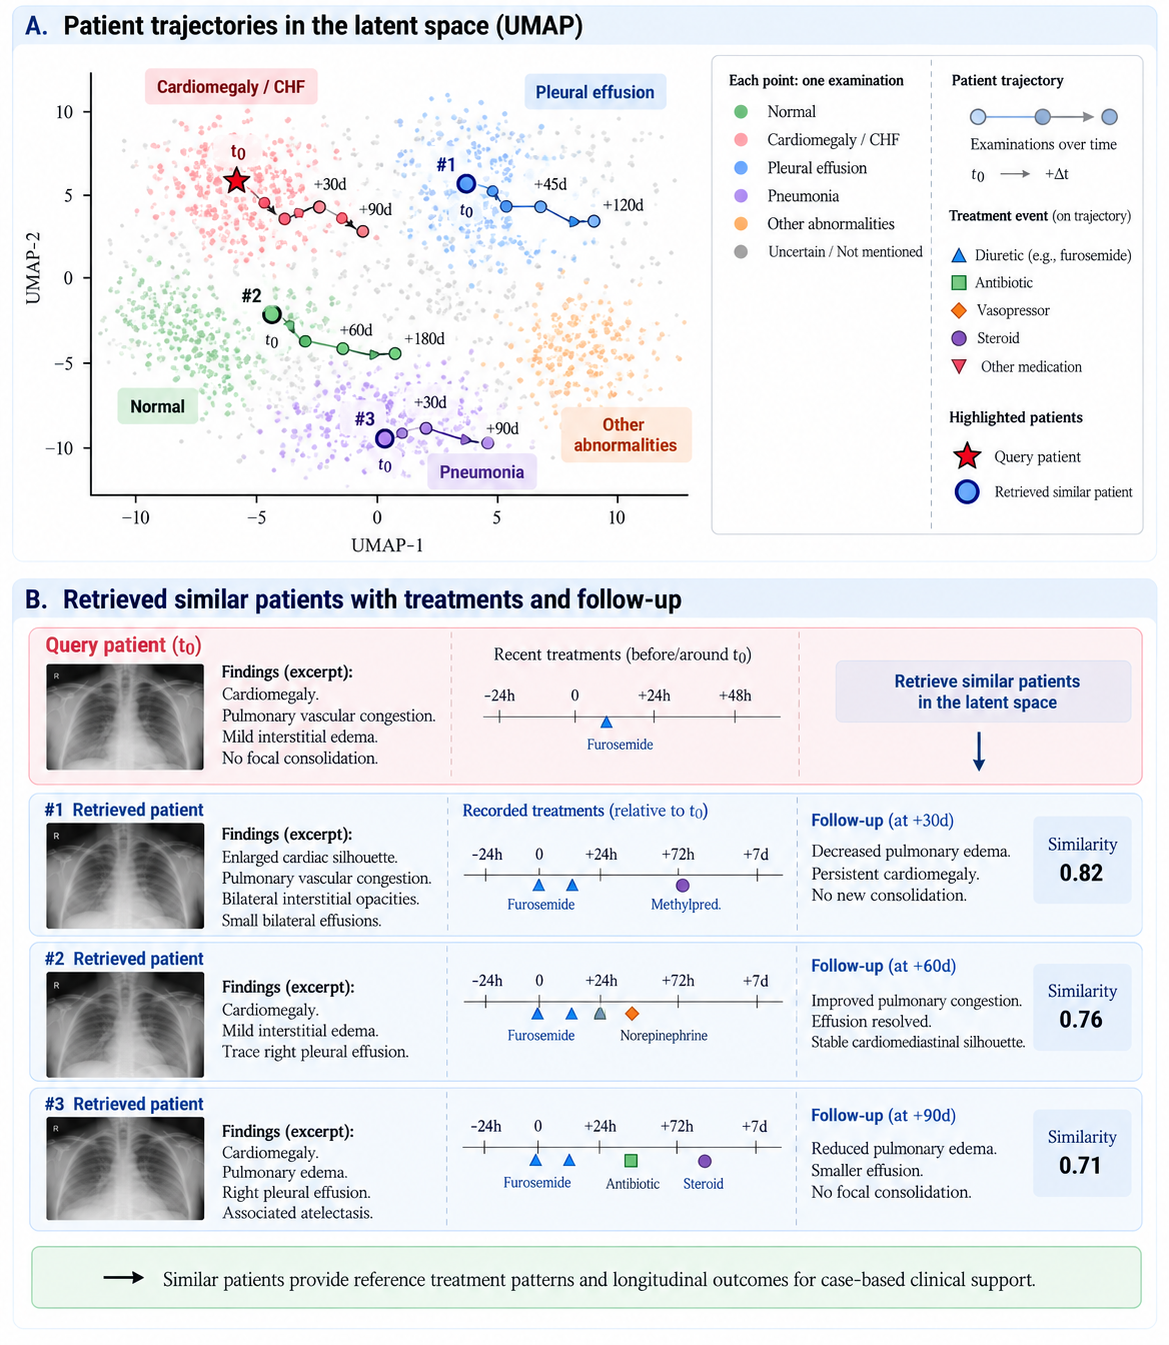
\includegraphics[width=\linewidth]{ppt/source/fig6_v1.png}
    \caption{\textbf{Patient state space and similar-case retrieval.}
    Planned visualization: (a) examination-level patient states with a query
    and its Top-3 matches, retrieved in the original representation space
    before projection; (b) the query and three distinct retrieved patients,
    showing current states and observed subsequent records. All examinations
    from the query patient are excluded. Follow-up information is used only
    for display; treatment entries require verified records.}
    \label{fig:candidate_patient_retrieval}
\end{figure}
